%!TEX root = ../../head.tex

\chapter{Übung}

\section{Einführung}
timo.schick@tu-dresden.de

\subsection{}
\begin{enumerate}
	\item Sterntopologie: Ein zentrales Element(Sternkoppler), jeder 				Rechner benötigt eine Leitung zu Sternkoppler \(\to\) 5
	\item Jeder mit Jedem \(= 4+3+2+1=10\)
	\item
	\begin{enumerate}
		\item \(l(n)= n\) bei Sterntopologie
		\item \(l(n) = \sum ... = (n*(n-1))/2\) bei vollvermaschter 					Topologie
	\end{enumerate}
	\item
	\begin{enumerate}
		\item LAN
		\begin{itemize}
			\item Reichweite: ~10m
			\item Reaktionszeit: niedrig
			\item Datenrate: hoch
			\item Topologien: Sterntopologie
		\end{itemize}
		\item MAN
		\begin{itemize}
			\item Reichweite: ~10km
			\item Reaktionszeit: mittel
			\item Datenrate: mittel
			\item Topologien: hierarchische Topologie
		\end{itemize}
		\item WAN
		\begin{itemize}
			\item Reichweite: ~100km - ~10.000km
			\item Reaktionszeit: hoch
			\item Datenrate: niedrig
			\item Topologien: Vollvermaschte Topologie
		\end{itemize}
	\end{enumerate}
\end{enumerate}

\subsection{}
\begin{enumerate}
	\item Dienst und Protokoll
	\begin{itemize}
		\item siehe Musterlösung
	\end{itemize}
	\item OSI Schichtenmodell
	\begin{itemize}
		\item Schichtenmodell siehe Folie 1.8ff
		\item Protokoll:
		\begin{itemize}
			\item ist eine Sprache zur horizontalen Kommunikation 							zwischen Prozessen derselben Schicht auf verschiedenen 						Hosts
		\end{itemize}
		\item Dienst
		\begin{itemize}
			\item dient der vertikalen Kommunikation zwischen zwei 							Schichten auf einem Host
		\end{itemize}
		\item Aufteilung des Bitstroms: Schicht 2 Sicherungsschicht
		\item Ende-zu-Ende Kommunkation: Schicht 4 Transportschicht
		\item Wegewahl: Schicht 3 Vermittlungsschicht
	\end{itemize}
	\item keine inhaltliche Bearbeitung, sondern nur 								Informationsweiterleitung
\end{enumerate}

\subsection{}
\begin{enumerate}
	\item
	\begin{itemize}
		\item siehe Folie 1.15; 
		\item Initiator (Prozess A), ...
		\item Responder (Prozess B), ...
	\end{itemize}
	\item
	\begin{enumerate}
		\item Zustände bestimmen
		\begin{itemize}
			\item idle
			\item connected
			\item prepare(Initiator)
			\item prepare(Responder)
		\end{itemize}
		\item Übergänge bestimmen (Knoten, Pfad, Knoten)
		\begin{itemize}
			\item (idle, conReq, prep(Init))
			\item (idle, ConInd, prep(Resp))
			\item (prep(Resp), conRsp, connected)
			\item (prep(Init), conCnf, connected)
			\item (connected, dataRep/dataInd, connected) 
			\item (prep(Resp)/prep(Init)/connected, disRep/disInd, idle)
		\end{itemize}
	\end{enumerate}
	\item
	\begin{enumerate}
		\item Ablaufdiagramm
		\begin{itemize}
			\item c1) + zeitlicher Ablauf
			\item c2) - es werden n Diagramme benötigt
			\item c3) - 
		\end{itemize}
		\item Zustandsdiagramm
		\begin{itemize}
			\item c1) - 
			\item c2) + alle Abläufe in einem Diagramm darstellbar
			\item c3) + 
		\end{itemize}
	\end{enumerate}
\end{enumerate}

\subsection{}
\begin{enumerate}
	\item siehe Folie 1.10
	\begin{enumerate}
		\item \(PDU(N)=SDU(N-1)\)
		\item \(IDU(N)=ICI(N)+SDU(N)\)
	\end{enumerate}
	\item Seitenaufruf: http://www.heise.de/software
	\begin{enumerate}
		\item httpRequest
		\begin{enumerate}
			\item  GET/software/http/1.1
			\item Host: www.heise.de
		\end{enumerate}
		\item ICI 
		\begin{enumerate}
			\item ip: 193.99.144.85 port:80
		\end{enumerate}
		\item SDU
		\begin{enumerate}
			\item  GET/software/http/1.1
			\item Host: www.heise.de
		\end{enumerate}
		\item IDU
		\begin{enumerate}
			\item ICI
			\item SDU
		\end{enumerate}
		\item TCP-PDU
		\begin{enumerate}
			\item src:80, dest:80,...
			\item SDU
			\item Data
		\end{enumerate}
	\end{enumerate}
	\item	
	\begin{align*}		
		b_{0}&=125\frac{\text{Mbit}}{\text{s}}\\
		b_{1}&=b_{0}\cdot0,8\\
		b_{2}&=b_{1}\frac{(55+99)0,01}2\\
		b_{3}&=b_{2}\frac{(57+99)0,01}2\\
		b_{4}&=b_{3}\frac{(23+99)0,01}2=36,4\frac{\text{Mbit}}							{\text{s}}\\
		b_{4}&=b_{goodput}\\
		b_{extra}&=b_{2}\frac{(23+99)0,01}2=46,7\frac{\text{Mbit}}						{\text{s}}
	\end{align*}
\end{enumerate}

\section{Bitübertragungsschicht}
\subsection{Nyquist-Theorem}
\begin{enumerate}
	\item 
	\begin{itemize}
		\item Bandbreite B [Hz]
		\item Signalrauschabstand SNR
		\item Abschneidefrequenzen in niedrigen Bereichen \(\to\) Differenz = Bandbreite
		\item Signalstufen S [1], digitaler Signal: \(S = 2\)
		\item Signalrate SR [Hz]
		\item Bitrate b \([\frac{\text{Bit}}{\text{s}}]\)
	\end{itemize}
	\(b = SR \cdot ld(S)\)
	\begin{itemize}
		\item Nyquist 1 (rauschfrei) \(b < 2\cdot B\cdot ld(2)\)
		\item Nyquist 2 (verrauscht) \(b < B \cdot ld(1+SNR) \)
		\item \(SNR_{dB} = 10 \cdot log_{10}(SNR)\)
	\end{itemize}
	Informationsgehalt \(I = ld(16) = 4 \text{ [Bit]f}\)\\
	Signalrate \(SR = \frac{b}{ld(S)} = \frac{9600 \frac{\text{ Bit}}{\text{s}}}{4 \text{ [Bit]}} \)
	\item
	\begin{align*}
	&SNR_{dB} = 12 \text{dB} \\ &SNR = 10^{\frac{SNR_{dB}}{10}} = 15 \\ &B > \frac{b}{(d(1+SNR))} = \frac{9600\frac{\text{Bit}}{\text{s}}}{ld(1+15)} = 2400 \text{Hz}
	\end{align*}
	\item 
	\begin{displaymath}
		B > 963 Hz \to B > 1200 Hz \text{Nyquist 1}
	\end{displaymath}
\end{enumerate}
\subsection{Pulsecodemodulation}
\begin{enumerate}
	\item
	\begin{itemize}
		\item PCM: analoges Signal \(\to\) Tiefpass \((f_{g}) \to \) Abtastung (zeitdiskret, \((f_{a})\)) \\ \(\to\) Quantisierung (wertdiskret)
		\item \(f_{a} > 2 f_{g}\)
	\end{itemize}
	gegeben: 
	\begin{align*}
		&B = 60 \text{ kHz} \\
		&QS = 1024 \\
		&S = 2
	\end{align*}
	gesucht:
	\begin{align*}
		b &< 2\cdot B \cdot ld(S) \\
		&= 2 \cdot 60\text{ kHz} \cdot 1\text{ [Bit]} \\
		&= \frac{120\text{ kBit}}{\text{s}}\\ \\
		f_{a} &= \frac{b}{(d(QS))}	\\
		&= \frac{b}{10\text{ [Bit]}} \\
		&= 12 \text{ kHz} \\
		f_{g} &< \frac{f_{a}}{2} \\
		&= 6 \text{ kHz}
	\end{align*}
	
	\item
	\begin{itemize}
		\item 8 Bit: leises Hintergrundrauschen
		\item 4 Bit: starkes Rauschen
		\item 1 Bit: extremes Rauschen
	\end{itemize}
\end{enumerate}
\subsection{Modulation}
\begin{enumerate}
	\item Tabelle zeichnen siehe VL
	\begin{enumerate}
		\item Amplitudenmodulation
		\item Frequenzmodulation
		\item Phasenmodulation
	\end{enumerate}
	\item 
	\begin{itemize}
		\item Realisierungsaufwand
		\begin{enumerate}
			\item sehr gut
			\item gut
			\item schlecht
		\end{enumerate}
		\item Störsicherheit
		\begin{enumerate}
			\item schlecht
			\item gut
			\item sehr gut
		\end{enumerate}
	\end{itemize}
\end{enumerate}
\subsection{Leitungskodierung}
\begin{enumerate}
	\item Leitungskodierung: \\Anpassung des Datenstroms an das eingesetzte Übertragungsmedium \\ 
	Ziel:
	\begin{itemize}
		\item Erkennung von Leitungsunterbrechungen
		\item Synchronisation (\(\to\) Takt)
	\end{itemize}
	\item einfacher Manchesterkodierung
	\begin{itemize}
		\item Leitungskode (Takt kann herausgelesen werden, Leitungen können unterbrochen werden)
		\item jedes Bit in zwei Intervalle teilen
		\item 0 \(\to\) low, high
		\item 1 \(\to\) high, low
	\end{itemize}
	\item siehe b)\\
	Übertragungsrate = \(\frac{1}{2}\) Signalrate
\end{enumerate}
\subsection{Multiplex}
\begin{enumerate}
	\item siehe Musterlösung
	\begin{itemize}
		\item synchrones Zeitmultiplex
		\begin{itemize}
			\item feste Zeitschlitze - Taktung nötig
			\item fester Zeitabschnitt für jeden Sender
			\item Zuordnung zu virtuellem Kanal durch Position im Übertragungskanal
		\end{itemize}
		\item asynchrones Zeitmultiplex
		\begin{itemize}
			\item feste Zeitschlitze - Taktung nötig
			\item Senden nach Bedarf
			\item Channel Identifier für Zuordnung zu virtuellem Kanal
		\end{itemize}
	\end{itemize}
	\item gegeben:
	\begin{align*}
		&B_{\text{Gesamt}} = 49 \text{ MHz} \\
		&B_{\text{Abstand}} = 1,5 \text{ MHz} \\
		&B_{\text{Kanal}} = 5,5 \text{ MHz}
	\end{align*}
	gesucht: Anzahl n der möglichen Fernsehkanäle:
	\begin{align*}
		&49 \text{ MHz} = 5,5 \text{ MHz} \cdot n + 1,5 \text{ MHz} \cdot (n - 1) \\
		&49\text{ MHz} = (5,5+1,5)\text{ MHz} \cdot n - 1,5 \text{ MHz} \\
		&50,5 = 7n \\
		&n = \frac{50,5}{7} = 7,21
	\end{align*}
	\(\to\) Es können 7 Kanäle angeboten werden.
\end{enumerate} 

\section{Netztechnologien 1}
\subsection{Ethernet}
\begin{enumerate}
	\item CSMA/CD
	\begin{enumerate}
		\item \(t_0\): A beginnt ein Frame zu senden
		\item \(t_0 + \tau - \epsilon\) B beginnt ein Frame zu senden
		\item \(t_0 + \tau \) B erkennt Kollision
		\item \(t_0 + \tau - \epsilon + \tau\) A erkennt die Kollision
	\end{enumerate}
	\(\Rightarrow t_s > 2\tau \) mit \(t_s\) Sendezeit für ein Frame
	\begin{align*}
	\tau &= \frac{d_{ges}}{v_{phy}}\\
	&= \frac{\text{|Repeater| }+1 \cdot d}{v_{phy}}\\
	&= \frac{5\cdot 500 \text{ m}}{\frac{200000 \text{km}}{s}}\\
	&= 12,5 \mu s\\
	&\rightsquigarrow 2\tau = 25 \mu s\\
	&\text{Sendezeit} = \frac{\text{Rahmenlänge}}{Bitrate}\\
	t_s &= \frac{F}{b}\\
	F &= t_s \cdot b > 2\tau \cdot b\\
	&= 25\mu s \cdot 10 \frac{\text{MBit}}{s}\\
	&= 250 \text{Bit}\\
	\end{align*}
	\item Ethernet Flow Control
	Switches kümmern sih um die Behandlung von potentiellen Kollisionen EFC dient ... siehe Lösungen
\end{enumerate}
\subsection{Switches}
	|Präambel (8)|Ziel (6)|Quelle (6)|Typ/Size (2)|\\Daten (1500)|CRC (4)|Interframe Gap (12)| \(\rightsquigarrow \) () in Byte
\begin{enumerate}
	\item Store-and-Foreward Switches \\
	\(t_s \text{ und } t_V\) werden vernachlässigt
	\begin{align*}
	&t_s + t_F + t_V + t_s + t_F\\
	t_F &= \frac{SL +F}{b} = \frac{(8+1518)\cdot 8\text{Bit}}{100 \cdot 10^6 \frac{\text{Bit}}{s}}\\
	&= 122,08 \mu s \\
	t_{ges} &= 4 t_F = 488,32 \mu s
	\end{align*}
	\item Virtual-Cut-Through Switches
	\begin{align*}
	&t_s + t_H + t_s + t_F\\
	t_{ges} &= 3t_H + t_F \\
	&= 122,08 \mu s + 3 \cdot \frac{14 \cdot 8\text{ Bit}}{100 \cdot 10^6 \frac{\text{Bit}}{s}}\\
	&= 122,08 \mu s + 3 \cdot 1,12 \mu s \\
	&= 125,44 \mu s
	\end{align*}
\end{enumerate}
\subsection{Transparent Bridges}
\begin{enumerate}
	\item Wegewahltabellen siehe Lösungen
	\item Bridge Informationen: \\
	X|Y : \\
	X = kommt von welchem Rechner, \\
	Y = kommt an welchem Port an
	\item Probleme 
	\begin{itemize}
		\item bei Zyklen (Pakete werden im Kreis weitergereicht
	\end{itemize}
	\item Spanning Tree Protocol
	siehe Lösungen
\end{enumerate}
\subsection{802.11 WLAN}
\begin{enumerate}
\item 
Wkt., dass ein Bit falsch ist: 
\begin{align*}
&e_{\text{Bit}} = 3 \cdot 10^{-6}
\end{align*}
Wkt., dass ein Bit richtig ist: 
\begin{align*}
&p_{\text{Bit}} = 1- e_{\text{Bit}}
\end{align*}
Rahmen mit 1500 Byte Größe:
\begin{align*}
&p_{Frame} = p_{Bit} \cdot \ldots \cdot p_{Bit} = (p_Bit)^{1500 \cdot 8} \\
&= (1-3\cdot 10^{-6})^{12000} = 0,96464 \\
e_{\text{Frame}} = 1-p_{Frame} = 0,035\\
\to \text{im Mittel 3,5 prozent der Frames fehlerhaft.}
\end{align*}
\item 
\begin{align*}
p_{Frame} &= (p_{Bit})^{(64\cdot 8)} = 0,99847\\
\to e_{Frame} &= 0,00153
\end{align*}
\end{enumerate}

\section{Netztechnologien 2}
\subsection{WiMax}
siehe Musterlösung
\subsection{RPR}
\begin{enumerate}
	\item Zeichnen Sie eine Topologie mit einem RPR Router pro Universität und den entsprechenden Ringlet-Verbindungen
	\item Abb.: \ref{img:RPR1}
	\begin{figure}
		\centering
		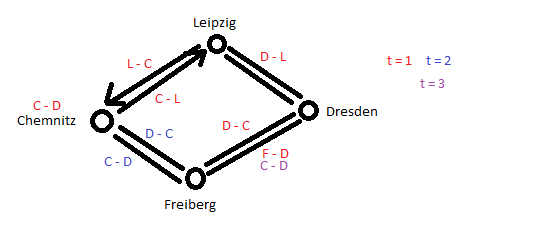
\includegraphics[width = 12cm]{./Rechnernetze/Images/4_2ab.png}
		\caption{RPR a) und b)}
		\label{img:RPR1}
	\end{figure}
	\item Abb.: \ref{img:RPR2}
	\begin{figure}
		\centering
		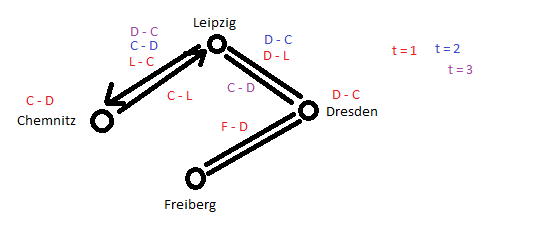
\includegraphics[width = 12cm]{./Rechnernetze/Images/4_2c.png}
		\caption{RPR c)}
		\label{img:RPR2}
	\end{figure}
\end{enumerate}
\subsection{Carrier Ethernet}
\begin{enumerate}
	\item Abb.: \ref{img:Netzaufbau}
	\begin{figure}
		\centering
		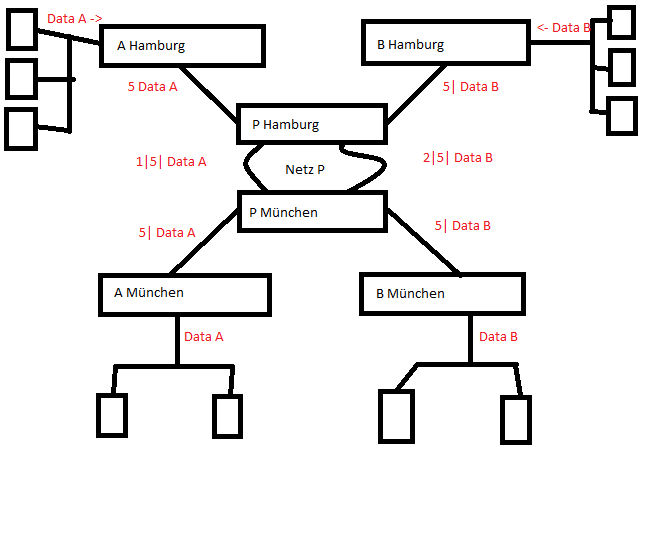
\includegraphics[width = 12cm]{./Rechnernetze/Images/4_3ab.png}
		\caption{Netzaufbau}
		\label{img:Netzaufbau}
	\end{figure}
	\item Abb.: \ref{img:Netzaufbau}
	\item Abb.: \ref{img:EthernetHeaderfeld}
	\begin{figure}
		\centering
		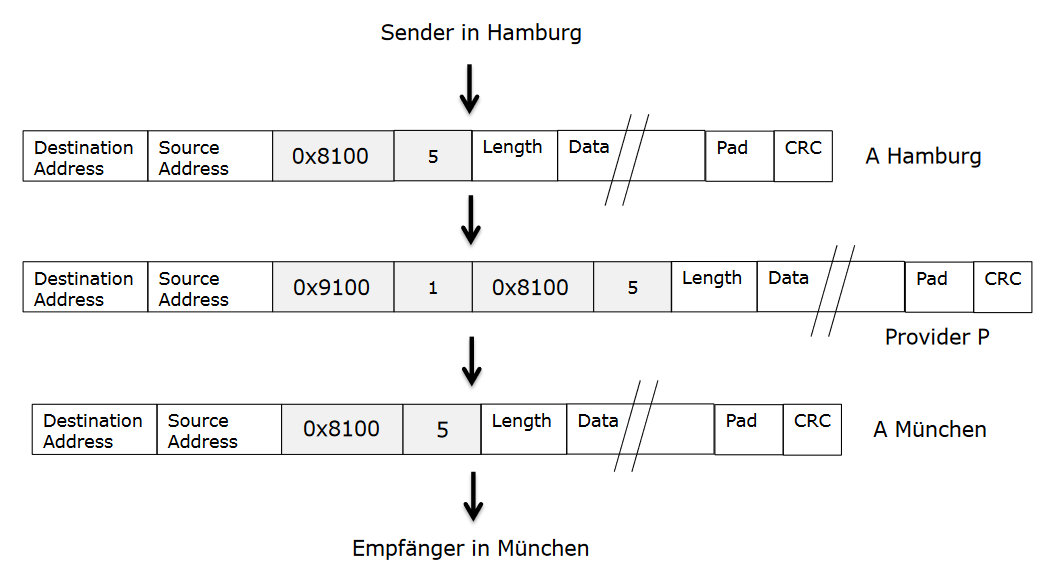
\includegraphics[width = 16cm]{./Rechnernetze/Images/4_3c.png}
		\caption{Ethernet Headerfeld}
		\label{img:EthernetHeaderfeld}
	\end{figure}
\end{enumerate}
\subsection{MPLS}
zu Abb.: \ref{img:MPLS} \\
\begin{tabularx}{\textwidth}{|X|X|X|X|r|}
\hline
	&\textbf{IN}	 	&\textbf{DEST}			&\textbf{OUT} &\\
\hline
\multirow{6}{*}{\textbf{SF}}
	&(1,-)	&134.5.0.0/16	&(3,1) &a)\\ 
	&(1,-)	&230.3.0.0/16	&(2,2) &a)\\
	&(2,7)	&*				&(1,-)	&c)\\
	&(3,10)	&*				&(1,-)	&c)\\
	&(1,-)	&134.5.42.0/24	&(2,11) &d)\\
	&(2,14)	&*				&(1,-)	&d)\\
\hline
\multirow{2}{*}{\textbf{H}}
	&(1,1)	&	&(3,4) &a) \\
	&(3,9)	&	&(1,10)&c) \\
\hline
\multirow{2}{*}{\textbf{W}}
	&(1,4)	&	&(3,5) &a)\\
	&(3,8)	&	&(1,)	&c)\\
\hline
\multirow{2}{*}{\textbf{C}}
	&(1,2)	&	&(2,3) &a)\\
	&(2,6)	&	&(1,7)	&c)\\
	&(1,11)	&	&(2,12)	&d)\\
	&(2,13)	&	&(1,14)	&d)\\

\hline
\multirow{2}{*}{\textbf{NY}} 
	&(2,5)	&*		&(3,-) &a)\\
	&(1,3)	&*		&(4,-) &a)\\
	&(4,-)	&217.8.0.0/16	&(1,6) &c) \\
	&(3,-)	&217.8.0.0/16	&(2,8)	&c) \\
	&(1,12)	&*		&(3,-)	&d)\\
	&(3,-)	&217.8.42.0/24	&(1,13)&d)\\
\hline
\end{tabularx}
\begin{figure}
		\centering
		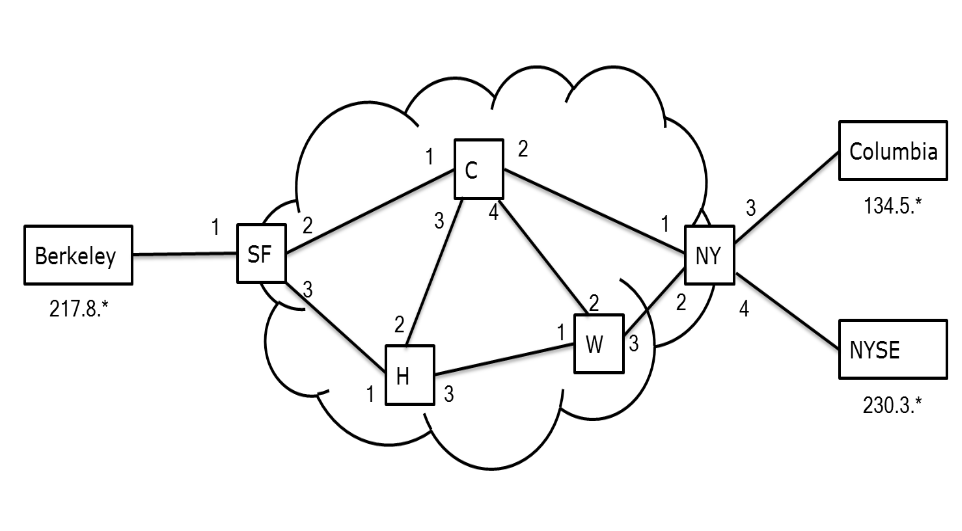
\includegraphics[width = 16cm]{./Rechnernetze/Images/4_4.png}
		\caption{MPLS-Network}
		\label{img:MPLS}
	\end{figure}
\begin{itemize}
	\item[b)] 
	\begin{tabularx}{\textwidth}{|X|X|X|}
	\hline
	Teilstrecke	&Label	&Ip-Dest \\
	\hline
	Berkeley - SF	&-	&134.5.20.217 \\
	\hline
	SF - H		&1	&134.5.20.217 \\
	\hline
	H - W		&4	&134.5.20.217\\
	\hline
	W - NY		&5	&134.5.20.217 \\
	\hline
	NY - Columbia	&-	&134.5.20.217 \\
	\hline
\end{tabularx}
\end{itemize}
\subsection{SONET/SDH und OTN}
Abb.:\ref{img:SONET}
\begin{figure}
		\centering
		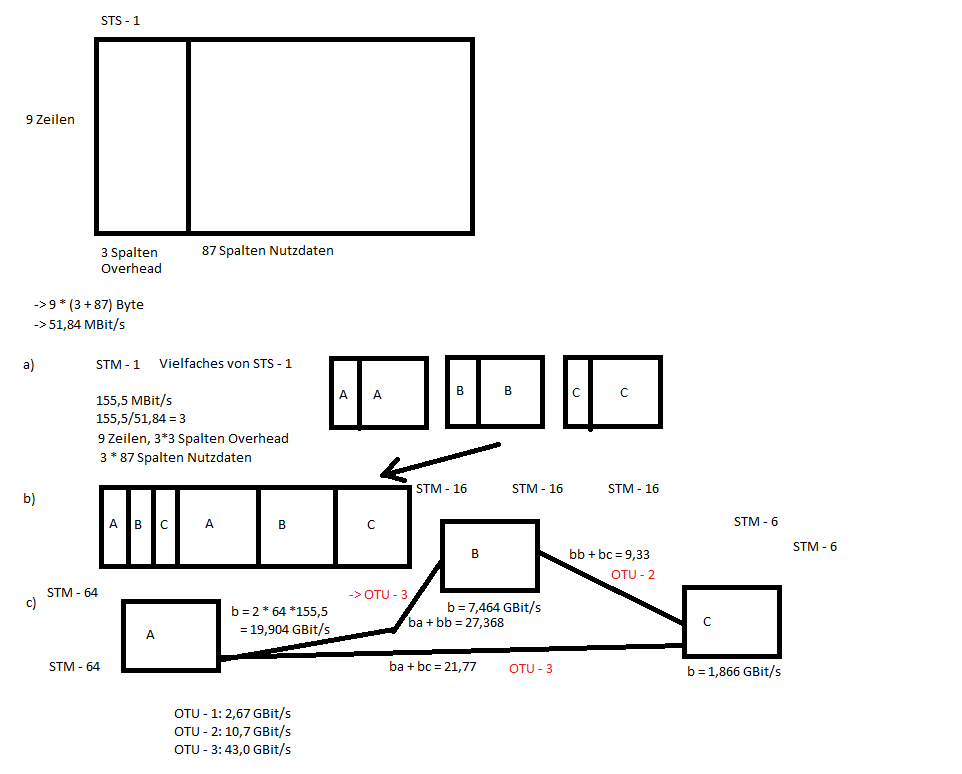
\includegraphics[width = 16cm]{./Rechnernetze/Images/4_5abc.png}
		\caption{STS - 1 und STM - N \((n \in \mathbb N)\)}
		\label{img:SONET}
\end{figure}